\section{Cronograma de Actividades, Demostración y Riesgos}\label{cap:cronograma}

\subsection{Cronograma general — Diagrama de Gantt}

El cronograma abarca dieciocho semanas, desde el lunes 2 de noviembre de 2026 hasta el domingo 7 de marzo de 2027. Al 16 de noviembre de 2026 el proyecto se encuentra en la semana 3, marcada con un asterisco. Las semanas 16 y 17 se reservan como margen para imprevistos, equivalentes al 11~\% del tiempo total, dentro del rango recomendado del 10~\% al 15~\%. El cronograma se amplió de catorce a dieciocho semanas porque la validación de instrumentos y la línea base retrospectiva no estaban contempladas en la versión anterior.


\begin{landscape}
\captionsetup{width=\linewidth}
{\footnotesize\setstretch{1.0}\setlength{\tabcolsep}{2pt}
\begin{longtable}{p{8.3cm}*{18}{>{\centering\arraybackslash}p{0.55cm}}}
\caption{Cronograma de actividades (18 semanas)}\label{tab:v4_6}\\
\toprule
\textbf{Actividad} & \textbf{S1}\newline{\tiny 02/11} & \textbf{S2}\newline{\tiny 09/11} & \textbf{S3*}\newline{\tiny 16/11} & \textbf{S4}\newline{\tiny 23/11} & \textbf{S5}\newline{\tiny 30/11} & \textbf{S6}\newline{\tiny 07/12} & \textbf{S7}\newline{\tiny 14/12} & \textbf{S8}\newline{\tiny 21/12} & \textbf{S9}\newline{\tiny 28/12} & \textbf{S10}\newline{\tiny 04/01} & \textbf{S11}\newline{\tiny 11/01} & \textbf{S12}\newline{\tiny 18/01} & \textbf{S13}\newline{\tiny 25/01} & \textbf{S14}\newline{\tiny 01/02} & \textbf{S15}\newline{\tiny 08/02} & \textbf{S16}\newline{\tiny 15/02} & \textbf{S17}\newline{\tiny 22/02} & \textbf{S18}\newline{\tiny 01/03} \\
\midrule\endfirsthead
\toprule
\textbf{Actividad} & \textbf{S1}\newline{\tiny 02/11} & \textbf{S2}\newline{\tiny 09/11} & \textbf{S3*}\newline{\tiny 16/11} & \textbf{S4}\newline{\tiny 23/11} & \textbf{S5}\newline{\tiny 30/11} & \textbf{S6}\newline{\tiny 07/12} & \textbf{S7}\newline{\tiny 14/12} & \textbf{S8}\newline{\tiny 21/12} & \textbf{S9}\newline{\tiny 28/12} & \textbf{S10}\newline{\tiny 04/01} & \textbf{S11}\newline{\tiny 11/01} & \textbf{S12}\newline{\tiny 18/01} & \textbf{S13}\newline{\tiny 25/01} & \textbf{S14}\newline{\tiny 01/02} & \textbf{S15}\newline{\tiny 08/02} & \textbf{S16}\newline{\tiny 15/02} & \textbf{S17}\newline{\tiny 22/02} & \textbf{S18}\newline{\tiny 01/03} \\
\midrule\endhead
\bottomrule\endfoot
\bottomrule\endlastfoot
1. Revisión bibliográfica (en curso) & \cellcolor{black!50} & \cellcolor{black!50} & \cellcolor{black!50} & \cellcolor{black!50} &  &  &  &  &  &  &  &  &  &  &  &  &  &  \\
2. Marco teórico y benchmarking (completado) &  & \cellcolor{black!25} & \cellcolor{black!25} &  &  &  &  &  &  &  &  &  &  &  &  &  &  &  \\
3. Diseño metodológico e instrumentos (borrador listo) &  &  & \cellcolor{black!50} & \cellcolor{black!50} &  &  &  &  &  &  &  &  &  &  &  &  &  &  \\
4. Validación de instrumentos por juicio de expertos &  &  &  & \cellcolor{black!75} & \cellcolor{black!75} &  &  &  &  &  &  &  &  &  &  &  &  &  \\
5. Línea base retrospectiva (registros del salón) &  &  &  &  & \cellcolor{black!75} & \cellcolor{black!75} &  &  &  &  &  &  &  &  &  &  &  &  \\
6. Cuestionario de requerimientos y entrevistas &  &  &  &  & \cellcolor{black!75} & \cellcolor{black!75} &  &  &  &  &  &  &  &  &  &  &  &  \\
7. Desarrollo del prototipo (MVP) &  &  &  &  & \cellcolor{black!75} & \cellcolor{black!75} & \cellcolor{black!75} & \cellcolor{black!75} & \cellcolor{black!75} &  &  &  &  &  &  &  &  &  \\
8. Piloto con el sistema (cuatro semanas) &  &  &  &  &  &  &  &  &  & \cellcolor{black!75} & \cellcolor{black!75} & \cellcolor{black!75} & \cellcolor{black!75} &  &  &  &  &  \\
9. Redacción del informe &  &  &  &  &  &  &  &  &  &  &  & \cellcolor{black!75} & \cellcolor{black!75} & \cellcolor{black!75} &  &  &  &  \\
10. Análisis de datos &  &  &  &  &  &  &  &  &  &  &  &  &  & \cellcolor{black!75} &  &  &  &  \\
11. Revisión y correcciones &  &  &  &  &  &  &  &  &  &  &  &  &  &  & \cellcolor{black!75} &  &  &  \\
12. Margen para imprevistos (dos semanas) &  &  &  &  &  &  &  &  &  &  &  &  &  &  &  & \cellcolor{black!10} & \cellcolor{black!10} &  \\
13. Presentación final &  &  &  &  &  &  &  &  &  &  &  &  &  &  &  &  &  & \cellcolor{black!75} \\
\end{longtable}}
\nota{Elaboración propia. S = semana; * semana en curso al 16 de noviembre de 2026. Gris muy oscuro: actividad planificada; gris medio: en curso; gris claro: completada; gris muy claro: margen para imprevistos.}
\end{landscape}

\subsection{Plan técnico complementario de ocho semanas}

Como ampliación para la materia de Soporte para la Toma de Decisiones, se plantea una ruta técnica complementaria de ocho semanas. Esta ruta no sustituye automáticamente el cronograma académico general de dieciocho semanas (Tabla~\ref{tab:v4_6}). Debe revisarse según la fecha real de la feria, el estado del repositorio y la disponibilidad de los integrantes. El alcance protege primero la exactitud financiera y después implementa un único ciclo DSS completo, antes de ampliar IA y automatizaciones.


\begin{figure}[H]
\caption{Cronograma técnico relativo de ocho semanas para el MVP DSS. S = semana; fechas exactas y disponibilidad por confirmar}\label{fig:dss_3}
\centering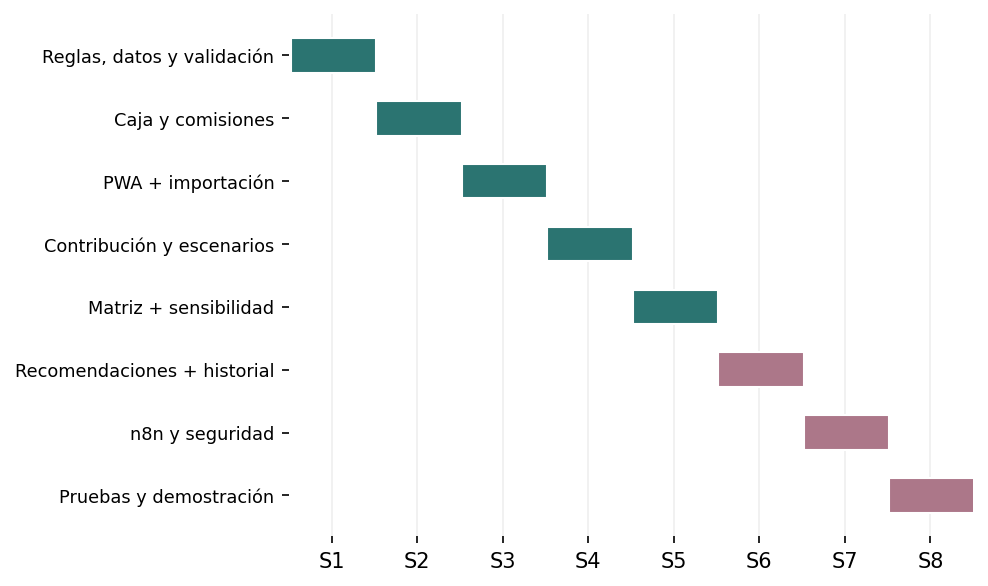
\includegraphics[width=0.9\linewidth]{img/fig_gantt_8sem.png}
\end{figure}

\subsubsection{Hitos y condiciones de salida}

\begin{vinetas}
\item S1: confirmar reglas, costos variables, casos de prueba, procedencia y restricciones de datos.
\item S2: asegurar motor de caja, ventas, cierres, comisiones y liquidación auditables.
\item S3: completar PWA offline e importación asistida con revisión humana.
\item S4: implementar contribución por servicio y escenarios What-If con cálculos de referencia.
\item S5: construir matriz multicriterio, ponderación, reglas de exclusión y sensibilidad.
\item S6: incorporar recomendaciones explicables, aprobación y seguimiento de decisiones.
\item S7: conectar notificaciones n8n a eventos aprobados y completar pruebas de permisos y seguridad.
\item S8: validar tareas decisionales, preparar datos sintéticos, documentar evidencia y ensayar demostración.
\end{vinetas}

\subsection{Guion de demostración ante el jurado}

La demostración ante el jurado seguirá una decisión central: ¿conviene aplicar una promoción del 10~\%? (1) Se muestra el Excel original con servicios inconsistentes; (2) se importa y valida información; (3) se registra una venta offline y se sincroniza sin duplicados; (4) el tablero calcula ingresos, comisiones y contribución; (5) el operador abre tres escenarios What-If y observa el volumen necesario para compensar el descuento; (6) Lush Decision Studio compara alternativas con criterios y sensibilidad; (7) Lush Insight explica la recomendación con evidencias y límites; y (8) la administradora aprueba o rechaza la propuesta y registra una revisión posterior. Como cierre opcional se muestra n8n generando una notificación de decisión aprobada, nunca una modificación automática de pagos.


\subsection{Riesgos y mitigaciones}

\vspace{8pt}{\small\setstretch{1.0}
\begin{longtable}{>{\raggedright\arraybackslash}p{0.3333\dimexpr\linewidth-6\tabcolsep\relax}>{\raggedright\arraybackslash}p{0.3333\dimexpr\linewidth-6\tabcolsep\relax}>{\raggedright\arraybackslash}p{0.3333\dimexpr\linewidth-6\tabcolsep\relax}}
\caption{Riesgos principales de la ampliación y acciones preventivas}\label{tab:dss_8}\\
\toprule
\textbf{Riesgo} & \textbf{Impacto} & \textbf{Tratamiento propuesto} \\
\midrule\endfirsthead
\toprule
\textbf{Riesgo} & \textbf{Impacto} & \textbf{Tratamiento propuesto} \\
\midrule\endhead
\bottomrule\endfoot
\bottomrule\endlastfoot
Alcance excesivo & MVP incompleto & Bloquear alcance crítico y priorizar vertical funcional \\
Pocos datos para ML & Predicciones inestables & Reglas primero; ML etiquetado experimental \\
LLM inventa cifras & Decisiones equivocadas & Herramientas cerradas, sin escritura, pruebas de referencia \\
Pérdida de conectividad & Ventas pendientes & Cola local, idempotencia y recuperación manual \\
Datos de nómina expuestos & Daño reputacional & Permisos, datos sintéticos, enlaces efímeros \\
Fallo de automatización & Avisos no entregados & Outbox, reintentos y seguimiento de errores \\
Cálculo de comisión ambiguo & Diferencia de liquidación & Firma/aprobación de políticas y snapshots \\
Tiempo limitado de feria & Demostración interrumpida & Entorno local, guion, contingencia y registro de video \\
Confundir simulación con predicción & Medio & Rotular supuestos, separar datos observados e hipótesis de volumen. \\
Recomendaciones por pesos arbitrarios & Medio & Validar pesos con administradora y mostrar sensibilidad. \\
Falta de costos de materiales & Medio & Mostrar contribución parcial y marcar faltantes; no afirmar utilidad neta. \\
Demasiados módulos DSS & Medio & Priorizar un solo caso de decisión completo con pruebas. \\
\end{longtable}}

\subsection{Estrategia de recorte y definición de terminado}

Si el tiempo disponible no permite terminar todas las funciones, se protegerá el ciclo de decisión completo: (a) exactitud del núcleo financiero; (b) cálculo de contribución; (c) simulación de tres escenarios; (d) matriz ponderada con sensibilidad y supuestos visibles; (e) recomendación explicable y aprobación humana; (f) historial de decisiones; (g) registro móvil, importación y un flujo n8n que apoyen la demostración. La IA generativa avanzada, las predicciones con ML y la optimización de capacidad podrán aplazarse. Una funcionalidad estará terminada solo cuando incluya interfaz usable, validación en backend, control de permisos, pruebas reproducibles y documentación suficiente para explicarla al jurado.

